\chapter{\IfLanguageName{dutch}{Stand van zaken}{State of the art}}
\label{ch:stand-van-zaken}

\section{Inleiding}
Dit hoofdstuk biedt een overzicht van de huidige stand van zaken rondom mobiele applicatieontwikkeling, met een focus op beveiliging, platformkeuze en cross-platform technologieën. Het doel is om de technologische context van dit project helder te krijgen en zo een gefundeerde keuze te maken voor .NET MAUI als ontwikkelplatform. Door recente ontwikkelingen en relevante literatuur te bespreken, leggen we een basis voor de daaropvolgende onderzoeksvragen en ontwerpkeuzes.

\section{Vergelijking van mobiele ontwikkelstrategieën}

Mobiele applicaties kunnen op verschillende manieren worden ontwikkeld, elk met hun eigen voor- en nadelen. De drie meest gangbare strategieën zijn: native apps, Progressive Web Apps (PWA's) en cross-platform frameworks. Deze sectie bespreekt elk van deze benaderingen afzonderlijk en vergelijkt ze vervolgens op het gebied van prestaties, gebruikservaring en ontwikkeltijd.

\subsection{Native apps}
Native apps worden specifiek ontwikkeld voor een bepaald platform, zoals Android of iOS, met gebruik van platformgebonden programmeertalen en tools zoals Kotlin of Java voor Android, en Swift of Objective-C voor iOS. Volgens \textcite{Bharadwaj2022} biedt deze benadering de beste prestaties en diepste integratie met het besturingssysteem, inclusief toegang tot hardwarecomponenten en native UI-elementen.

Een belangrijk voordeel van native ontwikkeling is de optimale gebruikerservaring. De app voelt aan als een natuurlijk onderdeel van het besturingssysteem, wat zorgt voor snellere laadtijden, vloeiendere animaties en consistente interactiepatronen \autocite{Pereira2024}. Daarentegen vereist deze strategie vaak twee aparte ontwikkelteams, wat leidt tot hogere ontwikkelkosten en langere time-to-market.

\textbf{Conclusie:} Native apps zijn ideaal wanneer maximale prestaties en diepe integratie vereist zijn, maar brengen hogere kosten en complexiteit met zich mee.

\subsection{Progressive Web Apps (PWA)}
Progressive Web Apps (PWA’s) zijn webapplicaties die functioneren als native apps door gebruik te maken van moderne webtechnologieën zoals HTML5, CSS3 en JavaScript in combinatie met service workers en manifest-bestanden \autocite{Osmani2023}. Ze worden uitgevoerd in een browseromgeving, maar kunnen offline functioneren, pushnotificaties sturen en op het startscherm van een toestel worden geïnstalleerd.

De belangrijkste voordelen van PWA’s zijn hun platformonafhankelijkheid en lage ontwikkelkosten. Eén codebase volstaat voor alle apparaten met een moderne browser. Echter, de functionaliteit van PWA’s is beperkter vergeleken met native apps, vooral op het gebied van toegang tot hardware en beveiligde APIs \autocite{Malavolta2023}. Op iOS bijvoorbeeld is de ondersteuning voor pushnotificaties en offline opslag nog steeds beperkt ten opzichte van Android.

\textbf{Kritische noot:} Hoewel PWA’s kostenbesparend zijn, blijven beperkingen in functionaliteit en platformondersteuning een uitdaging voor complexere applicaties.

\subsection{Cross-platform frameworks}
Cross-platform frameworks zoals Flutter, React Native en .NET MAUI bieden een compromis tussen de prestaties van native apps en de ontwikkelsnelheid van PWA’s. Deze technologieën maken het mogelijk om met één gedeelde codebase applicaties te ontwikkelen voor meerdere platforms, wat leidt tot een kortere ontwikkeltijd en lagere onderhoudskosten \autocite{Kuppan2024}.

Flutter en React Native renderen hun gebruikersinterfaces met behulp van eigen rendering-engines of native componenten, terwijl .NET MAUI gebruikmaakt van platform-native UI-elementen via .NET-technologie. Uit vergelijkend onderzoek blijkt dat Flutter uitblinkt in UI-prestaties en animaties, terwijl .NET MAUI voordeel biedt bij integratie in bestaande Microsoft-omgevingen \autocite{Gajjam2025}. Toch blijft de prestaties van cross-platform apps in sommige gevallen iets achter bij volledig native oplossingen, met name bij zware grafische of rekenintensieve toepassingen.

\textbf{Samenvattend:} Cross-platform frameworks bieden een aantrekkelijk evenwicht voor projecten met beperkte tijd en middelen, hoewel trade-offs in prestaties en integratie blijven bestaan.

\subsection{Vergelijking: prestaties, gebruikservaring en ontwikkeltijd}
De keuze voor een ontwikkelstrategie is vaak afhankelijk van de context, doelstellingen en technische randvoorwaarden van het project. In Tabel~\ref{tab:vergelijking-strategie} worden de drie besproken benaderingen vergeleken op basis van drie criteria: prestaties, gebruikservaring en ontwikkeltijd.

Native apps zijn ideaal voor toepassingen waarbij optimale prestaties en gebruikerservaring essentieel zijn, zoals games of applicaties met veel interactie. Voor eenvoudige toepassingen of informatieve apps kan een PWA volstaan. Cross-platform frameworks bieden een aantrekkelijk evenwicht voor projecten met beperkte tijd of middelen, zonder al te veel in te leveren op gebruikerservaring of prestaties \autocite{Longe2025}.

\section{Cross-Platform Ontwikkeling met .NET MAUI}

\subsection{Opkomst van .NET MAUI}
Een van de recente ontwikkelingen op het gebied van cross-platform mobiele ontwikkeling is de opkomst van .NET MAUI (Multi-platform App UI). Dit framework bouwt voort op eerdere technologieën zoals Xamarin en integreert nauw met het bredere .NET-ecosysteem, waaronder ASP.NET Core en Azure-diensten \autocite{Klesman2023}. In de literatuur wordt .NET MAUI vaak geprezen vanwege de verbeterde prestaties, moderne gebruikersinterface en de mogelijkheid om met één codebase apps te ontwikkelen voor meerdere platformen. Wanneer vergeleken met andere frameworks zoals React Native en Flutter, worden vooral de diepe integratie met Microsoft-technologieën en de schaalbaarheid als voordelen genoemd \autocite{Kuppan2024}.

\begin{figure}
	\centering
	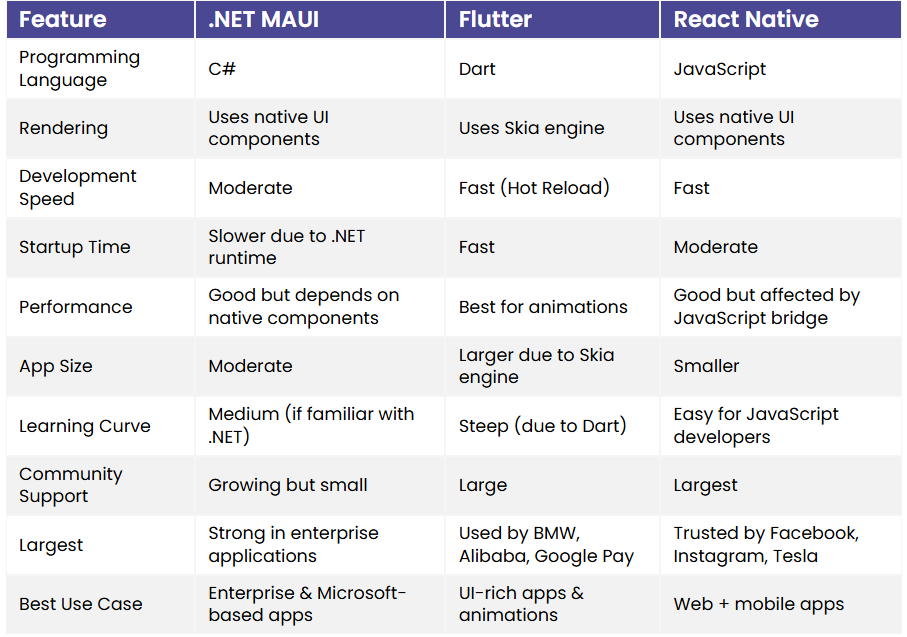
\includegraphics[width=0.8\textwidth]{comparison1.png}
	\caption[Integratie]{Geschiktheid van .NET MAUI voor enterprise-omgevingen}
\end{figure}

\subsection{Technologische Continuïteit}
Een belangrijke motivatie voor de keuze van .NET MAUI als ontwikkeltechnologie binnen dit project is de bestaande technologie-stack van de opdrachtgever, waarin reeds gebruik wordt gemaakt van het .NET-ecosysteem. Door .NET MAUI te verkiezen boven andere populaire cross-platform frameworks zoals React Native of Flutter, wordt er bewust gekozen voor technologische continuïteit en hergebruik van bestaande kennis en infrastructuur. Dit verlaagt niet alleen de leercurve voor ontwikkelaars, maar maakt ook integratie met bestaande backendcomponenten efficiënter, bijvoorbeeld via ASP.NET Core of Azure-integraties. Voor een organisatie die reeds vertrouwd is met C# en andere Microsoft-technologieën, vormt .NET MAUI daardoor een toekomstbestendige keuze die zowel technische als organisatorische voordelen oplevert \autocite{Longe2025}.

\textbf{Projectrelevantie:} Deze stand van zaken onderbouwt daarmee expliciet de keuze voor .NET MAUI binnen dit project.

\begin{figure}
	\centering
	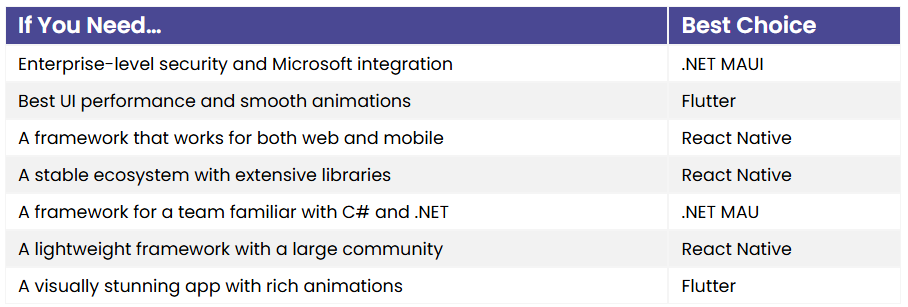
\includegraphics[width=0.8\textwidth]{comparison2.png}
	\caption[Vergelijking]{Vergelijking van cross-platform frameworks}
\end{figure}

\subsection{Vergelijking met Alternatieven}
Bovendien blijkt uit recente vergelijkende analyses tussen .NET MAUI, Flutter en React Native dat .NET MAUI bij uitstek geschikt is voor enterprise-omgevingen waarin stabiliteit, veiligheid en systeemintegratie centraal staan. Waar Flutter uitblinkt in UI-rijke toepassingen met vloeiende animaties, en React Native gewaardeerd wordt om zijn grote community en brede platformondersteuning, onderscheidt .NET MAUI zich door zijn native UI-componenten, nauwe integratie met Microsoft-tools zoals Visual Studio en Azure, en ondersteuning voor zowel desktop- als mobiele platformen. Deze eigenschappen maken het de meest geschikte keuze voor organisaties die vertrouwen op Microsoft-technologieën en op zoek zijn naar een eenduidige, schaalbare en onderhoudbare oplossing voor cross-platform applicatieontwikkeling \autocite{Gajjam2025}.

\textbf{Reflectie:} Toch zijn er nog uitdagingen, zoals het relatief jonge karakter van .NET MAUI en de afhankelijkheid van het Microsoft-ecosysteem, wat de flexibiliteit kan beperken in niet-Microsoft gerichte projecten.

\section{Moderne Authenticatie en Beveiligingspraktijken}

\subsection{Gebruik van JSON Web Tokens (JWT)}
Op het gebied van beveiliging signaleren onderzoekers een toenemende voorkeur voor moderne authenticatiemethoden. JSON Web Tokens (JWT) worden vaak genoemd als efficiënte en schaalbare manier om authenticatie en autorisatie te beheren in mobiele applicaties \autocite{Gao2023}. Deze tokens bevatten versleutelde gebruikersinformatie en stellen applicaties in staat om zonder server-side sessiebeheer toch een hoge mate van veiligheid te realiseren. JWT wordt gezien als een robuuste oplossing, mits correct geïmplementeerd, bijvoorbeeld met versleuteling, tijdsbeperking en verzending via beveiligde verbindingen.

\subsection{Wachtwoordbeveiliging}
Daarnaast blijft de veilige opslag van wachtwoorden een essentieel onderwerp binnen mobiele app-beveiliging. De toepassing van cryptografische hashing-algoritmes zoals bcrypt en PBKDF2 wordt breed aanbevolen vanwege hun weerstand tegen brute-force aanvallen \autocite{Gupta2022}. Het gebruik van salting als aanvullende techniek maakt dictionary-aanvallen moeilijker uitvoerbaar en is volgens de literatuur een noodzakelijke maatregel bij moderne wachtwoordbeveiliging \autocite{Arias2025}. Tegelijkertijd wordt in studies gewezen op de risico’s van verouderde algoritmes zoals MD5 en SHA1, die ondanks hun bekendheid vaak onvoldoende bescherming bieden \autocite{ReesCarter2024}.

\subsection{Beveiligde Login-interfaces}
De gebruikersinterface, en met name de loginpagina, wordt in de literatuur besproken als een kritiek punt waar gebruiksvriendelijkheid en veiligheid in balans moeten zijn. Beperkingen op het aantal mislukte inlogpogingen en het gebruik van tweefactorauthenticatie (2FA) worden genoemd als effectieve maatregelen om aanvallen zoals credential stuffing tegen te gaan \autocite{Chinnasamy2025, Jurisons2024}. Ook wordt het belang benadrukt van een goede gebruikerservaring, zodat beveiligingsmaatregelen geen hinder vormen voor legitieme gebruikers.

\textbf{Kritische reflectie:} Hoewel JWT en moderne hashing-technieken veel veiligheid bieden, blijft de implementatiecomplexiteit een risico, waarbij verkeerde configuraties tot kwetsbaarheden kunnen leiden.

\section{Beveiliging en Beheer van Pushnotificaties}

\subsection{Technische Implementatie}
Een ander belangrijk onderwerp binnen mobiele applicatieontwikkeling is het gebruik van pushnotificaties. Deze notificaties worden vaak gebruikt om gebruikers snel op de hoogte te brengen van belangrijke gebeurtenissen, bijvoorbeeld wanneer een app gekoppeld is aan systemen zoals zonnepanelen of slimme meters. In zulke situaties kunnen pushnotificaties gebruikers waarschuwen voor overproductie van energie of andere relevante veranderingen.

Bij het implementeren van pushnotificaties is een belangrijk technisch aspect het correct registreren en beheren van devicetokens. Voor iOS-apparaten kan worden gebruikgemaakt van Apple Push Notification Service (APNs), terwijl Android-apparaten kunnen gebruikmaken van Firebase Cloud Messaging (FCM). Bij het opstarten van een mobiele applicatie dient elk apparaat een uniek push-token aan te vragen. In het geval van Firebase gebeurt dit door per gebruiker een token te registreren dat aan zijn account wordt gekoppeld. Dit stelt de backend in staat om gerichte notificaties te versturen op basis van gebruikersacties of systeemgebeurtenissen.

\subsection{Beheer en Verificatie van Tokens}
Een aandachtspunt hierbij is de levensduur van deze tokens. Pushnotificatietokens kunnen vervallen, bijvoorbeeld bij herinstallatie van de app, verandering van instellingen of het verlopen van de sessie. Daarom is het van belang dat de applicatie in staat is om deze tokens automatisch te verversen en opnieuw te registreren bij de backend. In dit kader wordt vaak ook het automatisch vernieuwen van JWT-tokens op de achtergrond toegepast, zodat gebruikerssessies geldig blijven zonder handmatige interventie. Dit verhoogt niet alleen de veiligheid, maar ook de gebruikerservaring. Verder is het aan te raden om bij registratie het apparaattype (iOS of Android) mee te geven, zodat het systeem het juiste distributiekanaal voor notificaties gebruikt.

\subsection{Functionele Impact en Veiligheidsmaatregelen}
In de praktijk zullen gebruikers echter niet continu actief zijn binnen de mobiele applicatie. Dit betekent dat het geldig blijven van het pushnotificatietoken essentieel is: wanneer een token is vervallen of ongeldig is geworden, ontvangt de gebruiker geen meldingen meer – zelfs niet bij kritieke gebeurtenissen zoals het overschot aan opgewekte zonne-energie. In applicaties die afhankelijk zijn van realtime communicatie over belangrijke systeemstatussen, kan dit leiden tot functionele beperkingen of gemiste waarschuwingen.

Daarnaast moet bijzondere aandacht worden besteed aan de beveiliging van pushnotificatietokens en de inhoud van de berichten zelf. Pushnotificaties moeten voldoende gegevens bevatten om na ontvangst direct te kunnen navigeren naar de juiste pagina binnen de app, specifiek afgestemd op de juiste gebruiker en situatie. Dit betekent dat de notificatie bijvoorbeeld een gebruikers-ID of andere contextuele informatie moet bevatten. Omdat het hier vaak gaat om gevoelige gegevens, zoals energieverbruik of systeemstoringen, is het essentieel dat deze informatie op een veilige manier wordt verwerkt en verzonden, bijvoorbeeld via versleuteling of in combinatie met server-side verificatie bij het openen van de app via een notificatie. Een fout in dit proces kan leiden tot datalekken of ongeautoriseerde toegang tot persoonlijke informatie.

Wanneer een token vervalt, kan dit doorgaans worden opgevangen door de pushservice zelf, die een foutcode retourneert wanneer een bericht niet kan worden afgeleverd. Op basis hiervan kan het systeem het oude token verwijderen en bij de eerstvolgende gebruikersinteractie een nieuw token opvragen. Het implementeren van deze logica is essentieel om te waarborgen dat pushnotificaties betrouwbaar blijven functioneren over de gehele levenscyclus van de applicatie.

\textbf{Slotopmerking:} Beheer van pushnotificatietokens en beveiliging van notificaties zijn kritieke aandachtspunten die vaak onderschat worden, maar cruciaal zijn voor het succes van real-time mobiele applicaties.

